\section{Discussion}
\label{sec:disc}
\subsection{What the survey changes}
Laboratory cycle lives favour LFP strongly, and a model built on them finds LFP cheaper over ten years (by BDT \litGap{}). The survey reverses this. A lead-acid set costs BDT \costMedLA{} and is expected to last \replMedLA{} months; an LFP set costs \costRatio{} times as much but lasts only \replMedLFP{}/\replMedLA{} $\approx$ 2.4 times as long, and it resells for \scrapLFP\% of its price against \scrapLA\% for lead-acid. Per month of use the capital cost net of resale is about BDT 940 for lead-acid and BDT 1{,}940 for LFP, while LFP's electricity saving (\egLA{} $-$ \egLFP{} kWh per day) is only about BDT 360 per month at BDT 11.36/kWh. For an operator who pays the purchase price, lead-acid is the cheaper choice at present prices, which is consistent with its dominance in the sample. The result depends on LFP prices of 2026, on the replacement intervals drivers expect, and on five LFP respondents.

\subsection{What would make lithium replace lead}
Break-even requires either a lower LFP price (BDT \beP{} at the surveyed life, \bePpct\% below the median), a much longer life (\beL{} months at the surveyed price), or a combination (\figref{breakeven}). The tornado chart shows that the main uncertainties are the real life of lead-acid and of LFP sets and the LFP price, all of which can be pinned down by following drivers over time. The conclusion also changes if lead-acid sets fail faster than the survey median (8 months would roughly equalise the two), for instance under heavier loads or hotter batteries. For LFP to win without a price fall, operators would need a way to recover its higher resale value or spread its cost, for example leasing or battery swapping.

\subsection{Temperature: what matters and what does not}
Regional temperature does \emph{not} separate Khulna, Chuadanga and Rajshahi: mean battery temperatures differ by \Tspread\,$^\circ$C and the ranking is identical. Temperature acts through the seasonal cycle, heat waves and above all the battery's rise above ambient: moving it from 0 to 10\,$^\circ$C cuts lead-acid life from 23.8 to 12.5 months and LFP life from 51.6 to 35.3 months (Table~\ref{tab:scen}), but both chemistries are affected, so the cost ranking does not change. Heat-wave days age lead-acid faster (\heatLA{} times) than LFP (\heatLFP{} times). Measuring pack temperature in service is a higher priority than adding weather stations.

\subsection{Carbon: a smaller prize than lead, but robust}
A full switch saves about \fleetA{} Mt CO$_2$e per year at 1.4 M bikes, and the per-bike saving stays between \sensMin{} and \sensMax{} kg across the tested manufacturing footprints and grid factors. As the grid decarbonises the operational saving falls while the embodied saving remains. At BDT \abateCarbon{} per tonne CO$_2$e the carbon case alone is an expensive route to emission cuts; the case for LFP rests mainly on lead.

\subsection{Lead, workers and public health}
Used lead-acid batteries are collected, broken open and their lead plates smelted, often by hand and close to homes and farmland. Pure Earth describes informal recycling that contaminates and poisons workers and nearby residents \cite{pureearth_smep}, and ESDO identifies it as a primary contributor to lead-pollution hotspots \cite{esdo2021}. The IEDCR bulletin reports that about 36 million children (60\%) are poisoned by lead, that market screening in Dhaka, Rajshahi, Khulna and Barishal found 24\% of 197 consumer samples above reference lead levels, and that home assessments in 47 Khulna households found high lead in metal and ceramic cookware and toys \cite{das2026}. The World Health Organization notes that no safe level of lead exposure is known \cite{who_lead}. Remediation helps only partly: soil lead fell 96\% at an abandoned Savar site while child blood lead fell 35\% \cite{chowdhury2021}; the IEDCR bulletin reports a 20\% fall at Mirzapur, where hotspot soil dropped from about 100{,}000 ppm to 60--100 ppm \cite{das2026}; and a Tangail study reports 22\% \cite{eos2026}. Because blood lead falls much less than soil lead, other sources persist, so removing the source of new contamination is as important as cleaning old sites. Only 30\% of ULAB recycling is reported to be formal \cite{fe2024}, and UNCTAD estimates that about 80\% is informal and that 15--20\% of the lead recycled informally is released to the environment \cite{unctad_smep}. If the sixteen Powder users also run lead-based batteries, 88\% of the surveyed drivers do.

Our model supplies the \emph{quantity} side: LFP conversion removes \leadLow--\leadHigh{} kt of lead per year from the recycling stream at 1.4 M bikes (\figref{lead}), at an implied operator cost of BDT \abateLeadLow--\abateLeadHigh{} per kg of lead. It does not estimate how much of that lead would reach people; that needs emission and exposure data that do not yet exist, and other sources (paint, spices, cookware) also contribute.
\begin{figure}[t]
\centering
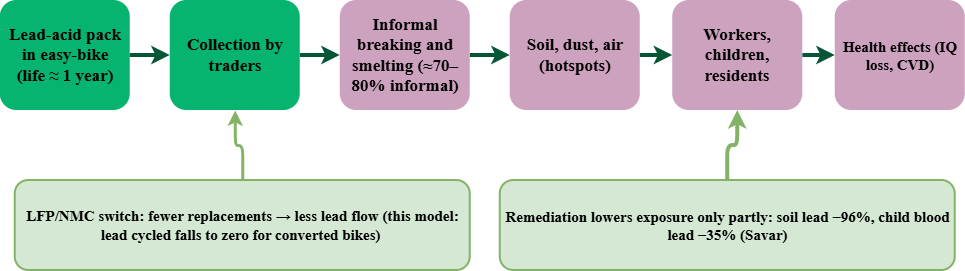
\includegraphics[width=0.9\textwidth]{fig_lead.png}
\caption{Pathway from lead-acid easy-bike batteries to exposure (schematic) and the point where an LFP switch acts; remediation figures from \cite{chowdhury2021}.}
\label{fig:lead}
\end{figure}

\subsection{Policy implications}
(i) \emph{Price and finance}: the BDT \premium{} premium and the BDT \gapLFP{} ten-year gap are barriers; leasing, pay-as-you-go and battery-swap schemes, or an import-duty cut that brings the LFP set below about BDT \beP{}, would close it. (ii) \emph{Support sized to the benefit}: full conversion of 1.4 M bikes needs about BDT \suppFull{} billion of support over ten years (Table~\ref{tab:policy}); this should be weighed against the health cost of lead, which is not in the model. (iii) \emph{ULAB regulation}: informal recycling is the main lead pathway, so licensed collection is a precondition for any lead benefit; the 2021 Hazardous Waste (e-waste) Management Rules reportedly cover household but not e-rickshaw lead batteries \cite{smep2024}. (iv) \emph{Lithium end of life}: a collection and recycling route must exist before volumes grow.

\subsection{Limitations}
\label{sec:limits}
\begin{itemize}
\item \textbf{Small convenience survey.} \nSurvey{} drivers, non-random, in the Khulna region; the LFP group has five respondents and four replacement answers, and these are expectations, not observed lifetimes. Several late-October entries have near-identical values, suggesting batch collection; excluding the ten from 27 October changes the lead-acid median from \replMedLA{} to \replLAnobatch{} months. \todo{[Insert survey locations and ethics statement.]}
\item \textbf{Calibration absorbs unknowns.} The fitted cycle lives (\NcalLA{} and \NcalLFP{}) also absorb operating days (not asked), charging practice and battery quality, and are not laboratory cycle lives.
\item \textbf{Equal pack size.} LFP capacity was not reported; it is set equal to the lead-acid Ah, and the LFP price is the median of sets of unknown capacity.
\item \textbf{Powder and charging cost.} Powder batteries (\nPW{} drivers) are not modelled because their chemistry is unconfirmed, and the charging-cost answers could not be pooled (per-charge, per-month and unspecified bases), so the tariff is taken from the BERC order and a hub-fee check.
\item \textbf{Energy use is from the literature}, not metered; the 52--88 Wh/km range is tested. The lead-acid pack runs above 80\% DoD at the survey distance.
\item \textbf{Cycle-limited life.} Calendar ageing is not modelled, and the LFP interval is an expectation.
\item \textbf{Vendor-level capacity curves, monthly temperature and an assumed battery temperature rise} (0--10\,$^\circ$C tested); hourly data would capture daily peaks.
\item \textbf{Scope.} NMC is not modelled because the survey contains no NMC users. Fire safety, weight and import dependence are not modelled, and lead flow is not exposure.
\item \textbf{Fleet size and tariff.} Fleet estimates range from 0.5 M autorickshaws to 4 M three-wheelers \cite{clean2024,pureearth_smep,unctad_smep}; the 3.0 M-bike results are an upper bound. The BDT 11.36/kWh rate is from press reports of the June 2026 BERC order \cite{berc2026fe,fenews2026}; tariffs of 7.70--16.24 change the gap by less than 15\%.
\end{itemize}
